\documentclass{beamer}
\usepackage{hyperref}
\usepackage[T1]{fontenc}

% other packages
\usepackage{latexsym, amsmath, mathtools, xcolor, multicol, booktabs, empheq}
\usepackage{graphicx,pstricks,listings,stackengine, datetime, subcaption}
\usepackage[skins,theorems]{tcolorbox}
\usepackage[font=scriptsize,labelfont=bf]{caption}
\usepackage[ruled,vlined]{algorithm2e}

\usepackage[backend=biber, bibstyle=ieee, citestyle=numeric-comp,
  sorting=none, labeldateparts,
  maxbibnames=99, maxcitenames=2, mincitenames=1]{biblatex} 

\newrobustcmd{\mkbibsubscript}[1]{%
  \unspace\allowhyphens\textsubscript{%
    \begingroup
    \protected\long\def\mkbibsuperscript##1{%
      \blx@warning{Nested superscript}%
      \mkbibbrackets{##1}}%
    #1\endgroup}}

\DeclareCiteCommand{\subcite}[\mkbibsubscript]
  {\usebibmacro{cite:init}%
   \let\multicitedelim=\supercitedelim
   \iffieldundef{prenote}
     {}
     {\BibliographyWarning{Ignoring prenote argument}}%
   \iffieldundef{postnote}
     {}
     {\BibliographyWarning{Ignoring postnote argument}}}
  {\usebibmacro{citeindex}%
   \usebibmacro{cite:comp}}
  {}
  {\usebibmacro{cite:dump}}

\addbibresource{ref.bib}

\author{Luca Polese}
\title{Landmark Graph-Based Indoor Localization \subcite{lgbil}}
\institute{Alma Mater Studiorum - Università di Bologna}
\newdate{date}{18}{06}{2024}
\date{\displaydate{date}}
\usepackage{Bologna}

% defs
\def\cmd#1{\texttt{\color{red}\footnotesize $\backslash$#1}}
\def\env#1{\texttt{\color{blue}\footnotesize #1}}
\definecolor{deepblue}{rgb}{0,0,0.5}
\definecolor{deepred}{rgb}{0.6,0,0}
\definecolor{deepgreen}{rgb}{0,0.5,0}
\definecolor{halfgray}{gray}{0.55}

\newcommand{\greent}[1]{\textcolor{deepgreen}{#1}}
\newcommand{\redt}[1]{\textcolor{deepred}{#1}}

\lstset{
    basicstyle=\ttfamily\small,
    keywordstyle=\bfseries\color{deepblue},
    emphstyle=\ttfamily\color{deepred},    % Custom highlighting style
    stringstyle=\color{deepgreen},
    numbers=left,
    numberstyle=\small\color{halfgray},
    rulesepcolor=\color{red!20!green!20!blue!20},
    frame=shadowbox,
}

\tcbset{highlight math style={enhanced, colframe=red!60!black, colback=white,arc=4pt, boxrule=1pt, drop fuzzy shadow}}

\NewEnviron{alignteo}{
  \begin{empheq}[box=\tcbhighmath]{align*}
  \BODY
  \end{empheq}
}

\DeclarePairedDelimiter{\abs}{\lvert}{\rvert}

\begin{document}

\begin{frame}
    \titlepage
\end{frame}

\section{Introduction}
\begin{frame}{\textbf{G}lobal \textbf{N}avigation \textbf{S}atellite \textbf{S}ystem}
    \begin{itemize}
        \item \textbf{GNSS} has been successfully applied in many fields:
    \end{itemize}
    \pause
    \begin{figure}[!htb]
        \centering
        \begin{subfigure}[b]{0.3\textwidth}
            \centering
            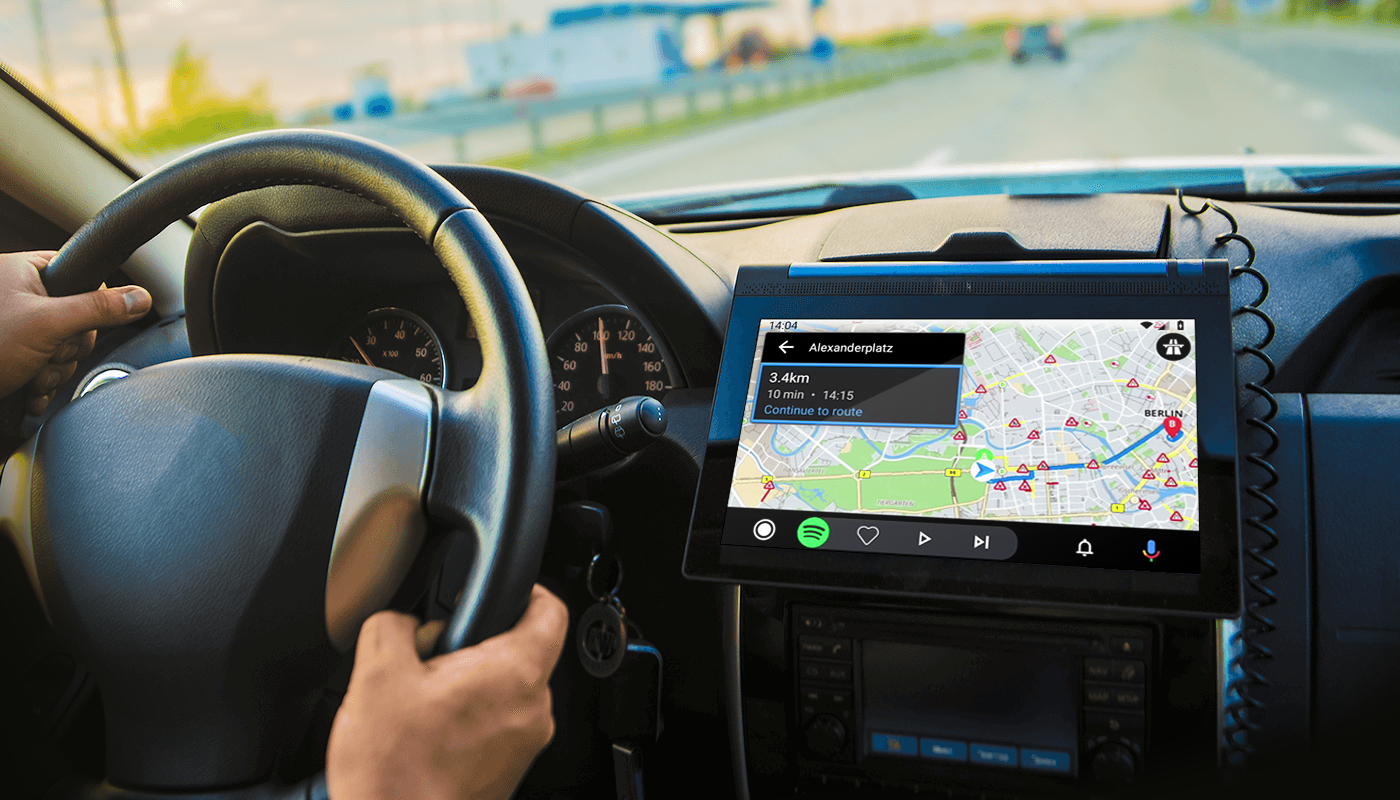
\includegraphics[width=\linewidth]{images/carnav.png}
            \caption{Car navigation}
            \label{fig:carnav}
        \end{subfigure}
        \hfill
        \begin{subfigure}[b]{0.3\textwidth}
            \centering
            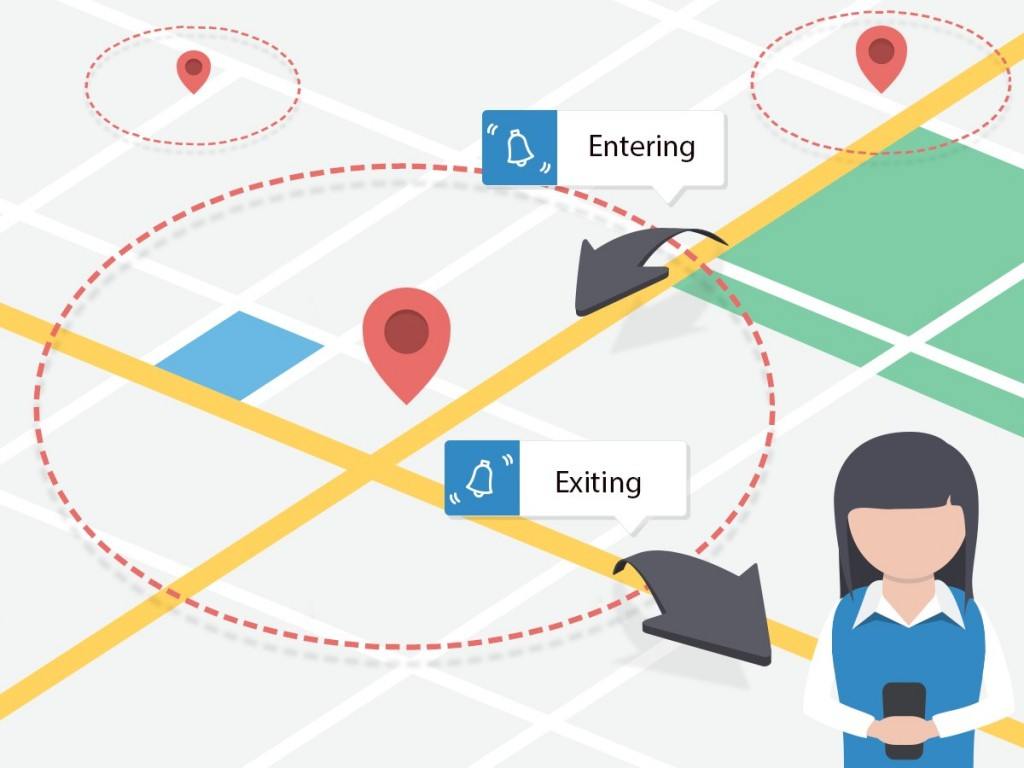
\includegraphics[width=\linewidth]{images/geofencing.jpg}
            \caption{Geofencing}
            \label{fig:geofencing}
        \end{subfigure}
        \hfill
        \begin{subfigure}[b]{0.3\textwidth}
            \centering
            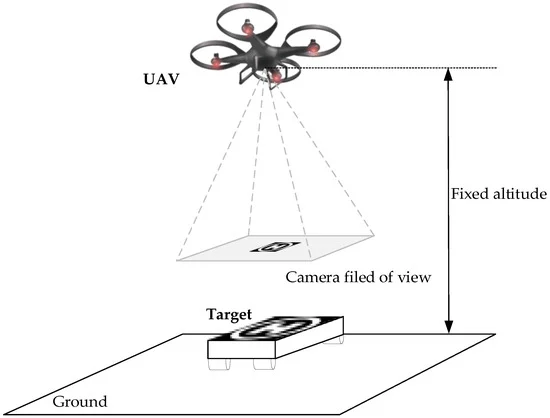
\includegraphics[width=\linewidth]{images/target.jpg}
            \caption{Target tracking}
            \label{fig:target}
        \end{subfigure}
           \caption{Some examples of application}
           \label{gnss}
    \end{figure}
    \pause
    \begin{itemize}   
        \item It's \textbf{difficult to use} for inside location: \textbf{signal} is \textit{blocked} by buildings, trees, obstacles, ...
    \end{itemize}
\end{frame}

\begin{frame}{Indoor localization}
    \begin{itemize}[<+->]
        \item It's even more \textbf{challenging}:
            \begin{itemize}
                \item Indoor spaces are more \textbf{complicated} in terms of \textit{layout}, \textit{topology}, \textit{space constraint};
                \item Indoor applications need more \textbf{accuracy}
            \end{itemize}
        \item Multiple systems have been proposed in recent years:
        \end{itemize}
        \pause
        \begin{figure}[!htb]
            \centering
            \begin{subfigure}[t]{0.24\textwidth}
                \centering
                
\includegraphics[width=\linewidth]{images/wifi.png}
                \caption{WiFi}
                \label{fig:wifi}
            \end{subfigure}
            \hfill
            \begin{subfigure}[t]{0.24\textwidth}
                \centering
                
\includegraphics[width=\linewidth]{images/zigbee.png}
                \caption{Zigbee}
                \label{fig:zigbee}
            \end{subfigure}
            \hfill
            \begin{subfigure}[t]{0.24\textwidth}
                \centering
                
\includegraphics[width=\linewidth]{images/bluetooth.png}
                \caption{Bluetooth}
                \label{fig:bluetooth}
            \end{subfigure}
            \hfill
            \begin{subfigure}[t]{0.24\textwidth}
                \centering
                
\includegraphics[width=\linewidth]{images/uwb.jpg}
                \caption{Ultra-wideband}
                \label{fig:uwb}
            \end{subfigure}
               \caption{Some examples of indoor localization systems}
               \label{indoor}
        \end{figure}
        \pause
        \begin{itemize}
        \item Each technique has \textbf{drawbacks} in terms of accuracy, cost coverage, complexity and applicability.
    \end{itemize}
\end{frame}

\begin{frame}{Hybrid methods}
    \greent{PRO}
    \pause
    \begin{itemize}
        \item Used to reach higher accuracy with relatively low cost
    \end{itemize}
    \pause
    \vspace{10pt}
    \redt{CON}
    \pause
    \begin{itemize}
        \item The required infrastructures may not be available in many environments or at a high cost
    \end{itemize}
\end{frame}

\begin{frame}{Spatial knowledge}
    \begin{itemize}[<+-| @alert +>]
        \item Available in many scenarios;
        \item It's used to assist localization without additional costs;
        \item Helpful for calibrating the localization error.
    \end{itemize}
\end{frame}

\begin{frame}{Landmark}
    \begin{block}{Definition of \textbf{landmark}}
        A \textbf{landmark} is generally defined in the field of linguistics and cognitive science as everything that stands out of the background.
    \end{block}
    \pause
    In the context of indoor localization, a landmark is 
    \begin{block}{Definition of \textbf{landmark} for indoor localization}
        A location point where at least one sensor presents a distinctive, stable  and identifiable pattern in the reading. Points are typically naturally distributed in indoor environments.
    \end{block}
\end{frame}


\begin{frame}
    \greent{PROS}
    \pause 
    \begin{itemize}[<+->]
        \item Location points are naturally distributed in indoor environments;
        \item So $\rightarrow$ localization error easy to bound if combined;
        \item No extra cost required.
    \end{itemize}
    \pause
    \redt{CONS}
    \begin{itemize}[<+->]
        \item Economically or/and computationally expensive;
        \item Systems that use laser scanner and/ora cameras to do so are not suitable for indo pedestrian localization;
        \item Performances rely highly on the completeness of landmarks;
        \item A mismatch of landmarks causes large localization errors (= failure of localization). 
    \end{itemize}
\end{frame}

\begin{frame}{LG-Loc}
    \begin{block}{Landmark-Guided Localization}
        It's a novel graph-based indoor localization method for smartphones
    \end{block}
    \pause
    Compared with existing landmark-based localization methods:
    \begin{itemize}[<+->]
        \item Computationally efficient;
        \item Handles incomplete landmarks;
        \item It uses landmarks to guide the localization process.
    \end{itemize}
    \pause
    \begin{block}{Landmark graph}
        It's a directed graph where nodes are landmarks and edges are accessible paths with heading information
    \end{block}
\end{frame}

\begin{frame}{LG-Loc $\sim$ Phases}
    This method consists of two phases:
    \pause
    \begin{enumerate}[<+->]
        \item \textit{offline}: data from several smartphones sensors are collected. With these data th initial landmark graph is constructed. We update the landmark graph by adding more landmarks;
        \item \textit{online}: newly collected data are used for location initialization, estimation and calibration.
    \end{enumerate} 
    \pause
    The initial location is inferred by a Hidden Markov model-based method and the location is regularly calibrated by matching the detected landmark with those in the landmark graph. 
\end{frame}

\begin{frame}{Challenges}
    \begin{enumerate}[<+->]
        \item Infer the initial location without manual input;
        \item Recognize landmarks satisfying;
        \item Deal with a landmark association issue and missing landmarks.
    \end{enumerate}
\end{frame}
\section{Related Works}
\begin{frame}{Indoor Localization $\sim$ Wifi-based}

	\greent{PROS}
	\begin{itemize}[<+->]
		\item Popular method that uses existing WiFi infrastructures, reducing deployment cost;
		\item Converts received signal strength (RSS) to distance for triangulation;
		\item Recent works use channel state information (CSI) for centimeter-level accuracy.
	\end{itemize}
	\pause
	\redt{CONS}
	\begin{itemize}[<+->]
		\item Low accuracy due to multipath effects in complex indoor environments;
		\item Requires knowledge of access point (AP) locations (difficult to obtain in public spaces);
		\item Fingerprinting methods based on RSS are time-consuming and
		\item CSI-based localization achieves high accuracy but has limited smartphone support.
	\end{itemize}

\end{frame}

\begin{frame}{Indoor Localization $\sim$ Dead Reckoning}
	\greent{PROS}
	\begin{itemize}[<+->]
		\item Uses inertial sensor readings for real-time location estimation of a target.
		\item No extra infrastructure required,
		\item Integration with other techniques (WiFi, UWB, vision) can improve accuracy.
	\end{itemize}
	\pause
	\redt{CONS}
	\begin{itemize}[<+->]
		\item It suffers from accumulated error: localization accuracy decreases over time;
		\item This leads to a long-term DR being useless.
	\end{itemize}
\end{frame}


\begin{frame}{Spatial Information-Aided Localization}

	\begin{block}{Spatial Information-Aided Localization}
		Spatial knowledge aids indoor localization without extra hardware costs.
	\end{block}
	\pause
	\begin{itemize}[<+->]
		\item \textbf{Landmark matching}: map matching method
		\item \greent{PROS}
			\begin{itemize}
				\item Simple \& high operation efficient.
			\end{itemize}
		\item \redt{CONS}
			\begin{itemize}
				\item Sensitive to landmark detection completeness;
				\item Inaccurate matching may lead to a larger localization error;
			\end{itemize}
		\item \textbf{Methods of Fusing Spatial Information}
		\item \greent{PRO}
			\begin{itemize}
				\item Includes richer information than basic indoor maps.
			\end{itemize}
		\item \redt{CON}
			\begin{itemize}
				\item Automated reconstruction methods are in early stages, manual methods are labor-intensive and slow.
			\end{itemize}
	\end{itemize}

\end{frame}

\section[L. Graph]{Landmark Graph}
\begin{frame}{Phase A $\sim$ Definition and Recognition of Landmarks}
    \begin{itemize}
        \item $\forall$ landmark $\exists$ 3 features:
            \begin{itemize}
                \item \textbf{Distinctiveness}: Unique patterns distinguishable from surroundings;
                \item \textbf{Stability}: It doesn't change dynamically over time;
                \item \textbf{Identifiability}: Detectable by one or more sensors.
            \end{itemize}
        \item Mathematical definition: \( v = \langle (x, y), (R_1, \ldots, R_M) \rangle \)
            \begin{itemize}
                  \item $(x, y)$: coordinate of the landmark;
                  \item $(R_1, \dots ,R_M)$: detection rule in different types of sensor readings;
                  \item $M$ is the number of rules that this landmark possesses.
            \end{itemize}
    \end{itemize}
\end{frame}

\begin{frame}{Types of Landmarks}
    \begin{columns}
        \begin{column}{.65\textwidth}
            \begin{itemize}[<+->]
                \item \textbf{Accelerometer Landmark}: Detects changes in \textbf{motion state};
                \item \textbf{Gyroscope Landmark}: Detects changes in \textbf{walking direction} using magnetometer \& gyroscope;
                \item \textbf{Barometer Landmark}: Measures \textbf{air pressure}, which changes with \textbf{altitude/height};
                \item \textbf{WiFi Landmark}: Detects location point that overhears the \textbf{strongest RSS from an AP};
                \item \textbf{Light Landmark}: Detects changes in \textbf{light intensity} using light sensor;
            \end{itemize}
        \end{column}%
        \hfill%
        \begin{column}{.35\textwidth}
            \begin{figure}[ht]
                \centering
                \includegraphics<1>[width=\linewidth]{images/racc.jpg}
                \includegraphics<2>[width=\linewidth]{images/rgyro.jpg}
                \includegraphics<3>[width=\linewidth]{images/rbaro.jpg}
                \includegraphics<4>[width=\linewidth]{images/rwifi.jpg}
                \includegraphics<5>[width=\linewidth]{images/rlight.jpg}
            \end{figure}
        \end{column}
    \end{columns}
\end{frame}

\begin{frame}{Phase B $\sim$ Construction of Initial Landmark Graph}
    \begin{itemize}
        \item Location of landmarks correspond to the \textbf{location of an element} inside the \textbf{floor map};
        \item The \textbf{landmark graph} is constructed starting from \textbf{map information}:
            \begin{itemize}
                \item \textit{Incomplete}: lacks room-level details (e.g., furniture, desks);
                \item Cannot locate WiFi and light landmarks from floor plan.
            \end{itemize}
        \item \textbf{Ingredients}:
            \begin{itemize}
                \item Nodes: Landmarks;
                \item Edges: Accessible paths between landmarks;
                \item Graph Representation: $G = (V, E)$:
                \begin{itemize}
                    \item $V$ = \{$v_1, \dots, v_N$\} (set of landmarks);
                    \item $E$ = \{$e_1, \dots, e_M$\} (set of edges).
                \end{itemize}
            \end{itemize}
    \end{itemize}
\end{frame}

\begin{frame}{Phase C $\sim$ Updating of Landmark Graph}
    \begin{itemize}
     
      \item \textbf{Learning New Landmarks}:
        \begin{itemize}
          \item Crowdsourcing: Collect $N$ user trajectories;
          \item Each trajectory contains $n_i$ potential landmarks \{$v_1^i, v_2^i, \dots, v_{n_i}^i$\}.
        \end{itemize}
      \item \textbf{Potential Landmarks}:
        \begin{itemize}
          \item Location points \textbf{satisfying} (at least) one \textbf{detection rule};
          \item \textbf{Not yet included} in the current \textbf{landmark graph}.
        \end{itemize}
      \item \textbf{Updating Algorithm}:
        \begin{itemize}
          \item \textit{Process}: Updates a landmark graph by \textbf{clustering potential landmarks} based on \textit{distance} and \textit{rules}, removing clusters with insufficient elements. Then ads new nodes and edges to the graph based on the cluster centers and detection rules.
        \end{itemize}
    \end{itemize}
\end{frame}


% \section[System]{System Overview}

\begin{frame}{LG-Loc System Architecture}
    \begin{columns}
        \begin{column}{.6\textwidth}
            \begin{itemize}
                \item Users launch the \textbf{localization application} upon entering a \textbf{building} and obtain their \textbf{location};
                \item Application requests the building's \textbf{landmark graph};
                \item Data used for \textbf{landmark detection} and \textbf{location estimation};
                \item Initial location obtained via:
                    \begin{itemize}
                        \item \textit{WiFi fingerprinting} (if database is \textbf{available});
                        \item \textit{HMM-based algorithm} (if database is \textbf{unavailable}).
                    \end{itemize}
            \end{itemize}
        \end{column}
        \begin{column}{.4\textwidth}
            \begin{figure}[t]
                \centering
                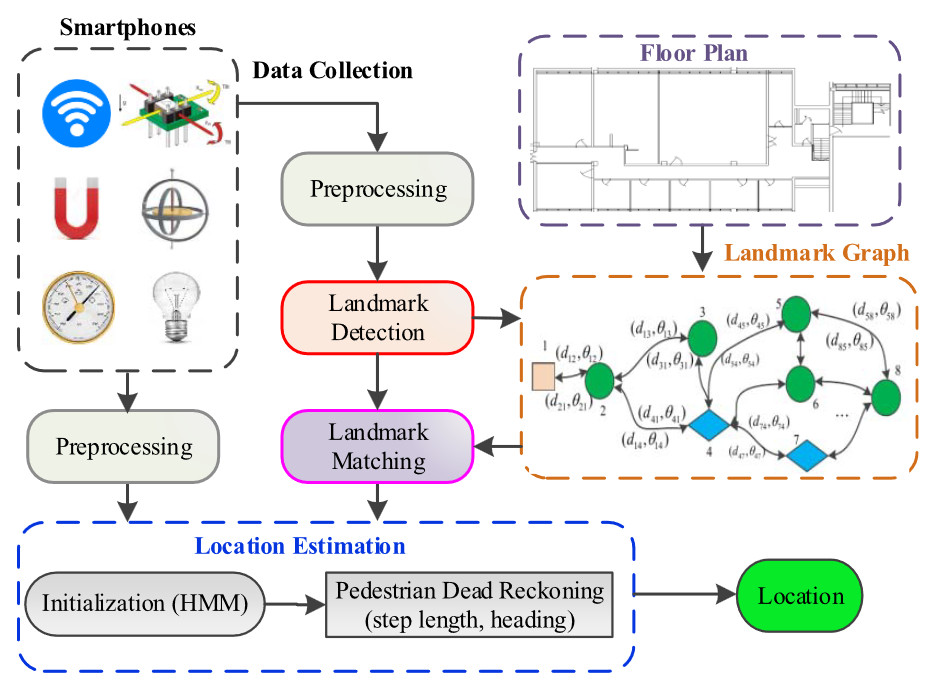
\includegraphics[width=\linewidth]{images/sys.jpg}
                \caption{System architecture of LG-Loc}
                \label{fig:sys}
            \end{figure}
        \end{column}
    \end{columns}
\end{frame}
% \section[L. Match]{Landmark Matching}
\begin{frame}{Challenges in Using Landmarks for Localization}
    \begin{itemize}
        \item \textbf{Relevant challenges to tackle}:
        \begin{itemize} 
            \item \textbf{Data Association Issue}: multiple landmarks nearby $\rightarrow$ difficult to determine the detected landmark;
            \item \textbf{Missing Landmarks}: Addressing cases where one or more landmarks are absent.
        \end{itemize}
        \item To solve the previous points a \textbf{belief} has been defined:
        \begin{itemize}
            \item Belief (\( bel \)): Indicates \textbf{trust level} that a location point \textbf{matches a landmark};
            \item Belief Calculation Formula:
            \[
                bel(v_k) = \highlight[tangerine]{\delta(R_k, R_t)} \cdot \highlight[cream]{r(\theta_k, \theta_t)} \cdot \highlight[sage]{g(d_k, d_t)}
            \]
        \end{itemize}
    \end{itemize}
\end{frame}


\begin{frame}{Functions Definitions}
    \begin{itemize}
        \begin{columns}
            \begin{column}{0.6\textwidth}
                \item Dirac Delta Function (\( \delta \)) for \textit{detection rule matching}:
                \item[] $ \!
                    \begin{aligned}
                        \highlight[tangerine]{\delta(R_k, R_t)} = \begin{cases}
                            1, & \text{if } R_k == R_t \\
                            0, & \text{otherwise}
                        \end{cases}
                    \end{aligned}
                $
                \item Rectangle Function (\( r \)) for \textit{heading comparison}:
                \item[] $ \!
                    \begin{aligned}
                        \highlight[cream]{r(\theta_k, \theta_t)} = \begin{cases}
                              1, & \text{if } |\theta_k - \theta_t| < \theta \text{ threshold} \\
                              0, & \text{otherwise}
                          \end{cases}
                    \end{aligned}
                $
                \item Exponential Distance Function (\( g \)) for \textit{distance comparison}:
                \item[] $ \!
                    \begin{aligned}
                        \highlight[sage]{g(d_k, d_t)} = e^{-|d_k - d_t|}
                    \end{aligned}
                $
            \end{column}
            \begin{column}{0.4\textwidth}
                \textbf{Landmark Selection and Error Correction}
                \begin{itemize}
                    \item Select the \textbf{landmark} with the \textbf{highest (\( bel \))};
                    \item Use (\( bel \)) threshold to \textbf{exclude fake landmarks};
                    \item \textbf{Ignore missing landmarks} and do not correct the location until the next landmark is detected.
                \end{itemize}
            \end{column}
        \end{columns}
    \end{itemize}
\end{frame}
% \section[Esteem]{Location Estimation}

\begin{frame}{Location Initialization}
    
    \textbf{Standard methods}
    
    \begin{itemize}
        \item \textit{WiFi Fingerprinting Method}:
            \begin{itemize}
                \item \textbf{Matches} new \textit{WiFi fingerprints} with a \textit{pre-collected database}
                \item Requires \textbf{offline training}, which is time-consuming and labor-intensive
            \end{itemize}    
        \item \textit{User Input Method}:
            \begin{itemize}
                \item User inputs \textbf{initial location} when launching the app
                \item Easy deployment but requires \textbf{active user participation}
            \end{itemize}
    \end{itemize}
    
    \textbf{Landmark Graph-based HMM Approach}
    \begin{itemize}
        \item Initially the app has no location information of the user;
        \item User walks to collect sensor readings for location estimation;
        \item Sensor readings used to fed the landmark recognition module;
        \item This way it generates observations to detect landmarks.
    \end{itemize}

\end{frame}
% \section[Results]{Experiments and Results}
\begin{frame}{Experimental Setup}
    \begin{itemize}
        \item \textit{Location}: Office building with eight floors;
        \item \textit{Environment}: Elevators, staircases, corridors, common rooms, office rooms;
        \item \textit{Testing path}: Two floors, approximately 362 meters long;
        \item \textit{Device}: Google Nexus 6 smartphone;
        \item \textit{Sensors}: WiFi, accelerometer, magnetometer, gyroscope, barometer, light sensor;
        \item \textit{Participants}: Six volunteers;
        \item \textit{Task}: Walk preset path, report markers for location accuracy.
    \end{itemize}
\end{frame}

\begin{frame}{Data Collection}
    \begin{block}{How the experient was carried out}
        The participants walked along the preset path with the phone in hand and reported the preset markers they encountered to evaluate the location accuracy.
    \end{block}
    \begin{itemize}
        \item Recorded data: \textbf{MAC addresses} of visible WiFi access points and \textbf{RSS};
        \item All data timestamped for alignment and inference;
        \item Participants clicked markers on Android app to set the locations.
    \end{itemize}
\end{frame}

\begin{frame}{Step Counting and Step Length Estimation}
    \begin{itemize}
        \item \textbf{Step counting step detection} and \textbf{step length} estimation have an impact on the \textit{accuracy of localization}: participants were asked to walk \textit{300 steps};
        \item Accuracy of step counting:
            \begin{itemize}
                \item Detection with/without constraints: > 94\%;
            \end{itemize}
        \item Step length estimation:
            \begin{itemize}
                \item Step length influenced by walking frequency (step periodicity);
                \item Step periodicity stability: Most steps in [0.5, 0.7] interval.
            \end{itemize}
    \end{itemize}
\end{frame}

\begin{frame}{Initial Location Determination}
    \begin{itemize}
        \item Ten random starting points along the path;
        \item Tested the HMM-based method to initialize th localization system;
        \item \textbf{Results}: Average distance a user has to travel to determine initial location is $\sim$ 9.95 m.
    \end{itemize}
\end{frame}

\begin{frame}{Numerical results}
    \settowidth{\leftmargini}{\usebeamertemplate{itemize item}}
    \addtolength{\leftmargini}{\labelsep}
    \begin{itemize}
        \item \textit{Performance}:
            \begin{itemize}
                \item \highlight[sage]{\textit{Proposed method}}: \textbf{88\% accuracy} with \textbf{error < 1.5 m};
                \item \highlight[cream]{\textit{Map filtering method}}: \textbf{63\% accuracy};
                \item \highlight[cream]{\textit{WiFi fingerprinting method}}: \textbf{33\% accuracy};
                \item \highlight[cream]{\textit{PDR methods}}: \textbf{Worst outcome} $\rightarrow$ lack of spatial constraints.
            \end{itemize}
        \item \textit{Mean error}:
            \begin{itemize}
                \item \highlight[sage]{\textit{Proposed method}}: \textbf{0.80 m};
                \item \highlight[cream]{\textit{Map filtering method}}: \textbf{$\sim$ 1.7 m};
                \item \highlight[cream]{\textit{WiFi fingerprinting method}}: \textbf{3.5 m};
                \item \highlight[cream]{\textit{PDR methods}}: \textbf{> 7 m}.
            \end{itemize}
        \item \textit{Efficiency} - comparison with \highlight[cream]{\textit{Map filtering method}}:
            \begin{itemize}
                \item $\sim$ 5 times faster;
                \item Landmark graph-based correction, no wall/obstacle detection;
                \item Suitable for resource-limited platforms.
            \end{itemize}
    \end{itemize}
\end{frame}
% \input{sections/Discussion.tex}
% \section{Conclusion}

\begin{frame}{Discussion on Landmark Graph-based Indoor Localization}
    
    \textbf{Achievements}
    \begin{itemize}
        \item Low-cost, robust, high accuracy (under 1 m);
        \item Reduces human effort for initial location input;
        \item Belief metric for accurate landmark matching.
    \end{itemize}
    
    \textbf{Conclusion}
    \begin{itemize}
        \item Novel, low-cost, high-accuracy indoor localization
        \item Sensor-based landmark detection with location correspondence
        \item Better accuracy and computational efficiency than existing methods
    \end{itemize}

    \texttt{ToDos}
    \begin{itemize}
        \item Sensor power consumption in smartphones;
        \item New thresholds for landmark detection: machine learning;
        \item Cooperation between multiple devices: exchange location and distance.
    \end{itemize}
    
\end{frame}

\section{Bibliography}
\begin{frame}{Bibliography}
    \printbibliography[heading=none]
\end{frame}

% \begin{frame}{Acknowledgments}
%     \begin{center}
%         {\Huge\calligra Thanks for the attention!}
%     \end{center}
% \end{frame}

\end{document}